%%%%%%%%%%%%%%%%%%%%%%%%%%%%%%%%%%%%%%%%%%%%%%%%%%%%%%%%%%%%%%%%%%%%%%
%% all the formatting stuff and packages

\documentclass[11pt]{article}

\parindent0em
\parskip.5em

\usepackage{xstring}

\usepackage{amsthm}
\usepackage[utf8]{inputenc}
\usepackage[ttscale=.85]{libertine}
\usepackage{libertinust1math}
% \usepackage[libertine,cmintegrals,cmbraces,vvarbb]{newtxmath}
\usepackage[T1]{fontenc}
\usepackage{microtype}
\usepackage{amsmath}
\usepackage{amssymb}
\usepackage{xspace}
\usepackage{ngerman}
\usepackage{graphicx}
\usepackage{lastpage}
\usepackage{ifthen}
\usepackage{fp}
\usepackage{hyperref}
\usepackage{icomma}
\usepackage{paralist}
\usepackage[ngerman,onelanguage,noend]{algorithm2e}
\DontPrintSemicolon

\makeatletter
\DeclareRobustCommand{\bfseries}{%
   \not@math@alphabet\bfseries\mathbf
   \fontseries\bfdefault\selectfont
   \boldmath
}
\makeatother

\usepackage[headsep=1cm]{geometry}

\usepackage{fancyhdr}

\fancypagestyle{plain}{%
  \renewcommand{\headrulewidth}{0pt}%
  \fancyhf{}
  \rhead{\includegraphics[width = 2.4cm]{fig/hpi_logo.pdf}}
  \lhead{\textbf{\sffamily Parametrisierte Algorithmen} \\
    \textbf{\sffamily Wintersemester 2017/2018} \\
    \sffamily Thomas Bläsius}
  \cfoot{\thepage}
  \rfoot{\ifthenelse{\thepage < \pageref{LastPage}}{\textit{bitte
        wenden}}{}}
}
\fancypagestyle{normal}{%
  \renewcommand{\headrulewidth}{0pt}%
  \fancyhf{}
  \cfoot{\thepage}
  \rfoot{\ifthenelse{\isodd{\thepage} \and \thepage <
      \pageref{LastPage}}{\textit{bitte wenden}}{}}
}

\usepackage{titlesec}

\titleformat{\section}%
[hang]%
{\Large\bfseries\sffamily}%
{Aufgabe \thesection:}%
{.5em}%
{}%
[]

\renewcommand{\thesubsection}{\alph{subsection}}
\usepackage{titlesec}
\titleformat{\subsection}%
[runin]%
{\bfseries\sffamily}%
{Teilaufgabe (\thesubsection)}%
{0pt}%
{}%
[]

\usepackage{titlesec}
\titleformat{\subsubsection}%
[hang]%
{\large\bfseries\sffamily}%
{\thesection}%
{.5em}%
{}%
[]

\titlespacing{\section}{0pt}{1.5ex}{.5ex}

\titlespacing{\subsection}{0pt}{.5ex}{.5em}

\titlespacing{\subsubsection}{0pt}{1ex}{.5ex}


%%%%%%%%%%%%%%%%%%%%%%%%%%%%%%%%%%%%%%%%%%%%%%%%%%%%%%%%%%%%%%%%%%%%%%
%% commands to use in the exercise sheet/solution

\newcommand{\sheet}[2]{ %
  \title{\textbf{\sffamily Übungsblatt #1}\\[-0.5ex]
    {\normalsize \sffamily Abgabe bis #2}}
  \date{}
  \maketitle
  \pagestyle{normal}
  \vspace{-2cm}
}

\newcommand{\solution}[2]{ %
  \title{\textbf{\sffamily Musterlösung zum Übungsblatt #1}\\[-0.5ex]
    {\normalsize \sffamily Erstellt von #2}}
  \date{}
  \maketitle
  \pagestyle{normal}
  \vspace{-2cm}
}

\newcommand{\exercise}[2][]{%
  \section{#2 \hfill {\normalsize#1}}%
}

\newcommand{\subexercise}{%
  \subsection{}%
}

\newcommand{\how}[1]{%
  \subsubsection*{Wie kommt man drauf?}%
}




\DeclareMathOperator{\vc}{vc}

\begin{document}

\solution{3}{Marvin Mirtschin, Tobias Stengel und Sören Tietböhl}

\exercise{Kreise der Länge 4}

\subexercise

$\varphi(X) = \forall e_1 = (v_1, v_2), e_2 = (v_3, v_4), e_3 = (v_5, v_6), e_4 = (v_7, v_8) \in E \colon \text{paarweiseVerschieden } \wedge (v_1 = v_8 \wedge v_2 = v_3 \wedge v_4 = v_5 \wedge v_6 = v_7) \rightarrow \{v_1, \dots, v_8\} \cap X \neq \emptyset$

Mit dieser $MSO_2$-Formel ist sichergestellt, dass sich mindestens ein Knoten jedes Kreises der Länge 4 in $X$ befindet.

Mit dieser Formel ist $|\varphi|$ konstant und damit liefert Courcelles Theorem einen FPT-Algorithmus in der Baumweite.
\how

Durch Courcelles Theorem wissen wir, dass es einen FPT-Algorithmus für das Problem gibt, wenn es sich in $MSO_2$ darstellen lässt.

Wir erstellen zunächst eine Formel, die prüft, ob ein Kreis der Länge 4 existiert. Ist das der Fall, muss durch die Formel sichergestellt werden, dass mindestens einer der betroffenen Knoten in der monadischen Variablen $X$ liegt, die unsere zu minimierende Menge repräsentiert.

\subexercise

Bei gegebener Baumweite $k$ lässt sich laut Theorem der Vorlesung (Foliensatz 5, Folie 14) eine Baumzerlegung der Weite $4k+4$ in $O(8^k\cdot k^2\cdot n^2)$ erstellen. Das liegt noch in der vorgegebenen Zeit von $O(2^{O(k^2)}\cdot n^{O(1)})$. Erstellen wir aus dieser Baumzerlegung eine schöne Baumzerlegung, können wir diese nun verwenden, um ein dynamisches Programm zu beschreiben:

Im weiteren betrachten wir $4k+4$ als neues $k$. Das können wir tun, weil das immer noch in $O(k)$ liegt. Zusätzlich zu den betrachteten Knoten eines Bags muss gespeichert werden, ob Paare von Knoten über einen vergessenen Knoten verbunden sind und somit noch einen Viererkreis bilden können.

Zunächst müssen alle Blätter der Baumzerlegung betrachtet werden. Es werden alle möglichen Kombination von in $X$ enthaltenen Elementen des Bags betrachtet. Wir wissen, dass es maximal $k+1$ Elemente im Bag geben kann, es gibt also $O(2^k)$ mögliche Kombinationen die Elemente aus dem Bag zu $X$ hinzuzufügen.

Anschließend müssen alle Kombinationen validiert werden, d.h. es muss geprüft werden, ob mit den entfernten Elementen der Bag keine Kreise der Länge 4 enthält. Wird noch ein Kreis gefunden, ist die geprüfte Kombination ungültig und kann somit aus der Ergebnismenge gelöscht werden. Diese Überprüfung auf Kreisfreiheit kann zum Beispiel mit BFS durchgeführt werden. Man führt eine Suche von jedem Knoten des $v_i$ Bags durch und merkt sich zusätzlich die Pfade zu gefundenen Knoten. Nach zwei Schritten kann dann abgebrochen werden. Findet man nach genau zwei Schritten von $v_i$ aus mindestens zwei mal den gleichen Knoten $u$ über unterchiedliche Pfade, ist ein Kreis gefunden, die Lösung also nicht valide.

Gehen wir nun von den Blättern der schönen Baumzerlegung zu den anderen Bags, muss die Menge der validen Kombinationen aktualisiert werden. Dafür gibt es Regeln für \textit{introduce-}, \textit{forget-} und \textit{join-}Knoten. 

Da Kreise eventuell über Knoten geschlossen werden, die nicht mehr im aktuellen Bag existieren, muss festgehalten werden, welche Knotenpaare potentiell in einem Kreis der Länge 4 enthalten sein können. Ein solches potentiell gefährliches Knotenpaar wird im weiteren als \textit{markiert} bezeichnet.

\begin{itemize}
\item[introduce: ]Beim Einfügen eines neuen Knotens $v$ wird entschieden, ob dieser in die Ergebnismenge $X$ aufgenommen wird oder nicht. Dazu wird zunächst geprüft, ob mit $v$ ein Kreis geschlossen wird, d.h. es wird geprüft, ob $v$ zu jedem Element eines markierten Knotenpaares eine Verbindung hat. Ist das der Fall, muss $v$ in $X$ aufgenommen werden. Es darf dann keine neue Teillösung erstellt werden, bei der $v\notin X$, da diese Teillösung einen Kreis der Länge 4 enthalten würde, ohne dass einer der vier Knoten in $X$ enthalten ist. Die Teillösung wäre damit invalide.

Andernfalls werden zwei Teillösungen erstellt. In einer ist $v\in X$, in der anderen nicht. Für die Teillösung, in der $v\in X$, ändert sich an den Markierungen nichts, da alle Kreise, die über $v$ geschlossen werden können durch $v\in X$ abgedeckt sind. In der anderen Teillösung ($v\notin X$) müssen neue Knotenpaare markiert werden. Zum einen müssen alle Knoten $u_i$, die eine Verbindung zu $v$ haben, paarweise miteinander markiert werden (s. \autoref{03-1b-markierung1}). Zum anderen müssen Paare ($v,u_i$) markiert werden, falls $v$ über einen anderen Knoten $w$ mit $u_i$ verbunden ist (s. \autoref{03-1b-markeirung2}). In beiden Teillösungen gilt, dass bisherige Markierungen unverändert bleiben, da eventuell andere Kreise über diese markierten Paare gebildet werden können.

\begin{figure}[h]
	\center
	%\subfig[asdf]{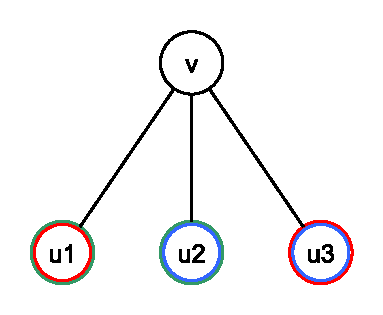
\includegraphics[scale=0.4]{fig/03-1b-markierung1}}
    %\subfig[asdf]{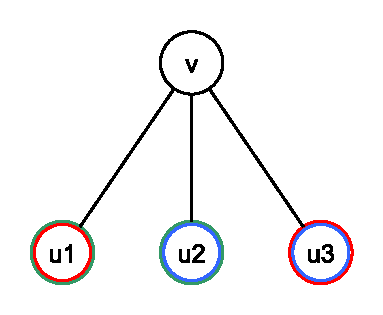
\includegraphics[scale=0.4]{fig/03-1b-markierung1}}
	\begin{minipage}{0.45\linewidth}
		\center
		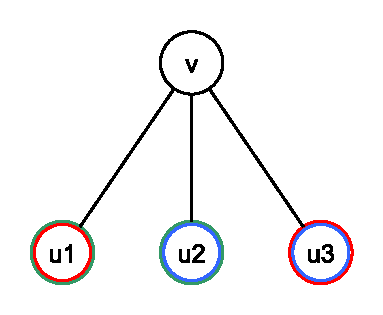
\includegraphics[scale=0.4]{fig/03-1b-markierung1}
		\caption{Paarweise Markierung über $v$}
		\label{03-1b-markierung1}	
	\end{minipage}	    
    \begin{minipage}{0.45\linewidth}
    	\center
		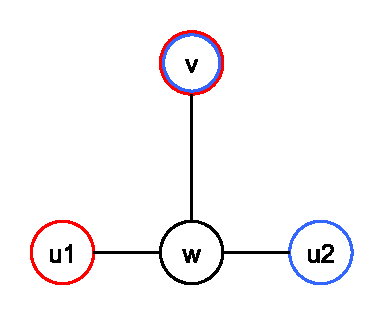
\includegraphics[scale=0.4]{fig/03-1b-markierung2}
		\caption{Markierung über $w$}
		\label{03-1b-markeirung2}	
	\end{minipage}	    
\end{figure}

Zu betrachten sind beim \textit{introduce} bis zu $k+1$ Knoten, welche bis zu $(k+1)^2$ Paare bilden können. Es müssen alle Knoten, zu denen der eingefügte Knoten eine Verbindung hat, paarweise markiert werden. Damit gibt es $O(k^2)$ neue Markierungen. Außerdem könnte jeder der $k$ Knoten mit dem eingefügten Knoten ein neues markiertes Paar bilden. Die Kosten für \textit{introduce} liegen somit in $O(k^2)$.

\item[forget: ]Beim vergessen eines Knoten $v$ müssen alle Markeirungen gelöscht werden, in denen $v$ Teil des Paares ist. Grund dafür ist, dass wir auf einer Baumzerlegung arbeiten und es daher keine Verbindungen von $v$ zu später eingeführten Knoten mehr geben kann.

Es gibt potentiell $k^2$ markierte Paare, die überprüft werden müssen, ob sie den Knoten $v$ enthalten. Die Kosten für \textit{forget} liegen damit in $O(k^2)$

\item[join: ] Beim Joinen von zwei Teilgraphen $G_1, G_2$ wird zunächst geschaut, ob ihre bisherigen Lösungen kombinierbar sind, d.h. ob sie die selben Knoten für $X$ gewählt haben. Somit wird sichergestellt, dass nur Teilgraphen gejoint werden, die in $X$ übereinstimmen.

Anschließend muss geprüft werden, ob es ein Knotenpaar $(u,v)$ gibt, das in beiden Teilgraphen markiert ist. Ist das der Fall, haben wir eine invalide Teillösung, da beim Zusammenführen von $G_1$ und $G_2$ ein Kreis der Länge 4 entsteht. Grund dafür ist, dass es in jedem der beiden Teilgraphen einen vergessenen Knoten $w_i$ gegeben haben muss, der $u$ und $v$ verbindet (s. \autoref{03-1b-join}). Da wir uns in einer Baumzerlegung befinden, muss für $w_1\in G_1, w_2\in G_2$ gelten, dass $w_1\neq w_2$. Die Teillösung muss also nicht weiter verfolgt werden. Gibt es kein Knotenpaar, das in beiden Teilgraphen markiert ist, müssen die Mengen der in den Teilgraphen markierten Knoten vereinigt werden. Die Teillösung wird danach weiterverfolgt.

\begin{figure}[h]
	\center		
	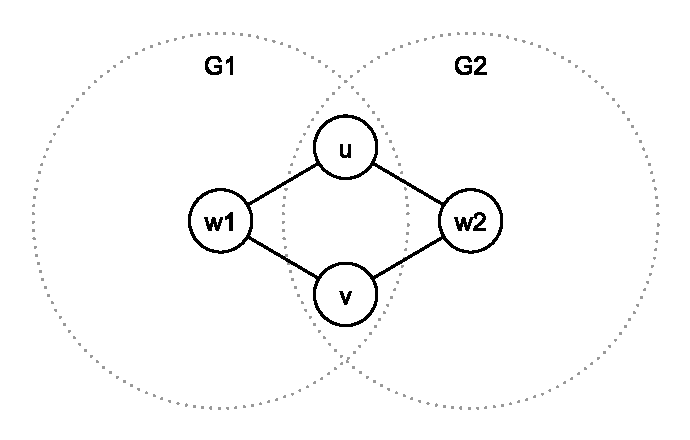
\includegraphics[scale=0.5]{fig/03-1b-join}
	\caption{Kreisentstehung beim \textit{join}}
	\label{03-1b-join}
\end{figure}

Für jede der $k^2$ Markierungen im ersten Teilgraphen muss geprüft werden, ob es diese Markierung auch in der Menge der $k^2$ Markierungen im zweiten Teilgraphen gibt. Die Kosten für \textit{join} liegen damit in $O(k^4)$.
\end{itemize}

Es gibt $O(2^k)$ mögliche Teillösungen, die mithilfe von \textit{introduce}, \textit{forget} und \textit{join} aktualisiert werden müssen. Die teuerste Operation davon (\textit{join}) liegt in $O(k^4)$. Die Anzahl der Bags der Baumzerlegung liegt in $O(n)$. Damit ergeben sich Gesamtkosten von $O(2^k\cdot k^4\cdot n)$ für den Algorithmus.

\how

Die gegebene Laufzeit der Aufgabenstellung lässt darauf schließen, dass ein Teil des Algorithmus ($2^{O(k^2)}$) darin besteht, von einer Menge mit $O(k^2)$ Elementen alle möglichen Teilmengen betrachten müssen.

Da die Baumweite $k$ gegeben ist, scheint es eine gute Idee zu sein, eine (schöne) Baumzerlegung zu erstellen, da dort jeder Bag nur noch $O(k)$ Elemente enthält. Da $2^{O(k^2)}$ gegeben ist, können davon auch alle möglichen Paare betrachtet werden. Der von $n$ abhängige Teil der Laufzeit ($n^{O(1)}$) erlaubt es uns über alle Bags zu iterieren, da die Anzahl dieser in $O(n)$ liegt.

Mit dieser Baumzerlegung kann nun ein dynamisches Programm erstellt werden. Dabei orientieren wir uns an der Idee zum Finden eines Hamiltonkreises (s. Foliensatz 3 Folie 11ff.) mithilfe der Baumzerlegung. Wir machen es uns zum Vorteil, dass die unerwünschten Kreise die konstante Länge 4 haben. Wir führen die Markierung von Knotenpaaren ein, um zu speichern, ob zwei Knoten je ein Ende eines Pfades der Länge 3 repräsentieren, um beim Einfügen eines neuen Knotens zu prüfen, ob sich ein Kreis der Länge 4 schließt.

\exercise{Chordale Graphen}

\subexercise
\label{sec:sep-clique}

Sei $G = (V,E)$ ein chordaler Graph sowie $a,b \in V$ zwei verschiedene, nicht-adjazente Knoten. Sei $S$ ein inklusionsminimaler Separator, der $a$, und $b$ trennt.
Wir nehmen im folgenden an, dass $S \neq \emptyset$, denn sonst gibt es nichts zu zeigen. Das bedeutet, dass $a$ und $b$ in derselben Zusammenhangskomponente liegen.

Daraus folgt erstmal direkt, dass $$\forall s \in S \, \exists p = (s, \dots, b) \colon (s' \in S \wedge s' \in p \rightarrow s = s') \wedge a \notin p$$

Es gibt also von jedem Knoten im Separator aus einen Weg zu $b$ der nicht über $a$ oder einen anderen Separatorknoten $s'$ führt.
Das gleiche gilt analog für vertauschtes a und b.

Ersteres bedeutet einfach nur, dass der Weg ein Teilpfad von $a$ nach $b$ ist und der Separator tatsächlich ein Separator ist. Für den zweiten Teil schauen wir uns das Gegenteil an:
Mal angenommen, es gibt keinen Pfad von $s$ aus, der nicht über einen anderen Knoten von $S$ führt. Dann ist $S$ nicht inklusionsminimal, denn wir könnten $S \setminus \{s\}$ bilden und hätten einen gültigen Separator.

Betrachten wir nun mal die konstruierte Situation als Graph.

\begin{center}
    \vspace{1ex}
    \includegraphics[page=1]{fig/03-2a-pfade}
\end{center}

Wir haben mind. zwei Knoten $s_1$ und $s_2$, die im Separator liegen.

Es führen Pfade von a zu beiden Knoten. Diese Pfade müssen nicht wie im Bild dargestellt knotendisjunkt sein, aber das erleichtert die Vorstellung.

Von $s_1$ und $s_2$ gibt es die oben beschriebenen Pfade nach $b$, die keine anderen Knoten des Separators verwenden. Auch diese Pfade müssen nicht knotendisjunkt sein.

Allerdings gibt es hiermit mindestens 4 Knoten, die einen Kreis der Länge mind. 4 induzieren. Im Beispielbild sind das $a, s_1, b, s_2$. Falls die Pfade nicht knotendisjunkt sind, wählen wir anstatt von $a$ und $b$ einfach die letzte Stelle, an der sich die entsprechenden Pfade einen Knoten teilen.

Der Graph kann also nur dann chordal sein, wenn es eine Kante zwischen $s_1$ und $s_2$ gibt. Da die Knoten beliebig aus $S$ gewählt sind, gilt dies für alle Knoten aus $S$.
(Anmerkung: zwischen $a$ und $b$ kann es keine Kante geben, da $S$ ja der Separator ist)
Demnach müssen die Knoten aus S also eine Clique bilden.

\how

Die Herleitung ist sehr direkt. Man konstruiert die Ausgangssituation, d.h. wählt sich zwei Knoten und den Separator und überlegt dann, wie man hier einen Kreis mit Länge 4 konstruieren kann.
Das geht nur, wenn zwei Knoten im Separator nicht miteinander Verbunden sind. Demnach muss dieser also eine Clique bilden.

\subexercise

Wir führen den Beweis per Induktion über die Anzahl der Knoten im Graphen.

\textbf{$i = 1$:}
Der Graph mit einem Knoten ist trivialerweise eine Clique.

\textbf{Induktionsvorraussetzung:}
Die Aussage des Satzes gilt für alle $k = (0, \dots, i)$

\textbf{$i \rightarrow i + 1$:}

Sei $C = (V,E)$ mit $|V| = i + 1$ ein chordaler Graph.
Entweder $C$ ist eine Clique, oder es gibt Knoten $v_1, v_2$ die nicht adjazent sind.

Im ersten Fall sind wir fertig, denn es gibt in einer Clique auch keine zwei nicht-adjazenten Knoten. Im zweiten Fall verfahren wir wie folgt:
Sei $S$ ein inklusionsminimaler Separator, der $v_1$ und $v_2$ trennt.
$S$ teilt den Graphen in zwei Teile $A$ und $B$, wobei $S$ nach Teilaufgabe \ref{sec:sep-clique} eine Clique bildet:

\begin{center}
    \vspace{1ex}
    \includegraphics[page=1]{fig/03-2b-sep}
\end{center}

Jetzt können wir die Induktionsvorraussetzung auf beide Teile $A \cup S$ und $B \cup S$ anwenden.
Es gibt zwei Möglichkeiten:

\begin{itemize}
	\item [Fall 1:] $A \cup S$ ist eine Clique. Dann wählen wir einen beliebigen Knoten aus $A$.
	\item [Fall 2:] Es gibt zwei nicht-adjazente simpliziale Knoten in $A \cup S$. Da $S$ eine Clique ist, können nicht beide Knoten in $S$ liegen. Wir wählen den Knoten, der in $A$ liegt.
\end{itemize}

Dasselbe machen wir analog für $B \cup S$ und haben somit zwei nicht adjazente simpliziale Knoten in $C$ gefunden.

\how

Unsere erste Idee war es, erst einmal zwei nicht adjazente Knoten zu nehmen, und dann zu zeigen, dass entweder die gewählten Knoten simplizial sind, oder man sich an den Nachbarn entlanghangeln kann, bis man bei einem Knoten ankommt der simplizial ist.
Das hat in einer sehr komplizierten Fallunterscheidung gemündet. Vor allem das induktive Argument des 'entlanghangelns' war schwierig zu beweisen.

Induktion war aber schon ein Schritt in die richtige Richtung. Teilaufgabe \ref{sec:sep-clique} beschäftigt sich mit Separatoren, und wenn wir uns an Aufgabe 3 von Blatt 2 erinnern, ist das Vorgehen ähnlich.

Man teilt den Graphen mit einem Separator und betrachtet dann die übriggebliebenen Teilgraphen vereinigt mit dem Separator.
Dann muss man nur noch die Induktion anwenden.

\end{document}
